Dopo aver montato il circuito in Figura \ref{fig:Circuit} si è proseguito con la regolazione del potenziometro visualizzando sull'oscilloscopio il segnale di uscita del battito cardiaco, che riportato in Figura \ref{fig:hearth-graph}. Il segnale $V_0$ del circuito è stato connesso all'ingresso analogico A0 della scheda Arduino DUE. Si è collegato il pin del diodo LED IR all'uscita digitale 6 e il diodo LED ROSSO all'uscita digitale 7. Per l'analisi della frequenza cardiaca si è utilizzato solamente il LED rosso.
\begin{figure}[H]
    \centering
    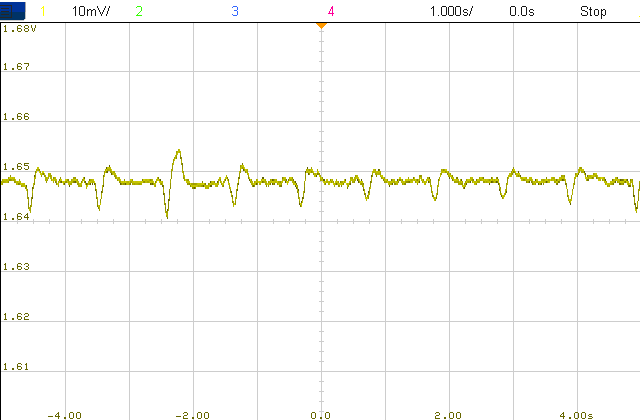
\includegraphics[width=.7\linewidth]{scope_3.png}
    \caption{Segnale del battito cardiaco}
    \label{fig:hearth-graph}
\end{figure}
\subsection{Codice acquisizione}
Scrivere un codice che permetta di acquisire il segnale in uscita al cardiofrequenzimetro, graficandolo sul display TFT allo stesso tempo.
\begin{lstlisting}[frame=single, language=Arduino]
#include <SPI.h>
#include "Adafruit_GFX.h"
#include "Adafruit_HX8357.h"
#define sensorPin A0
#define PinIR 6
#define PinRED 7
#define TFT_CS 10
#define TFT_DC 9
Adafruit_HX8357 tft = Adafruit_HX8357(TFT_CS, TFT_DC,-1); 
const int dispWidth = 480;
const int arraySize = dispWidth;
const int graphHeight = 200;
const int sampleInterval = 20;
int acquire[arraySize];
\end{lstlisting}
\clearpage
\begin{lstlisting}[frame=single, language=Arduino]
void setup(){
    pinMode(PinIR,OUTPUT);
    pinMode(PinRED,OUTPUT);
    analogReadResolution(12); // 12 bit ADC -> 4096 values

    digitalWrite(PinRED,HIGH); // Acceso con anticipo per adattare il circuito di filtraggio
    
    tft.begin();
    tft.setRotation(3);
    tft.fillScreen(HX8357_BLACK);
    tft.setTextSize(3);
    tft.setCursor(30, graphHeight);
    tft.setTextColor(HX8357_WHITE);
    tft.println("Heart Rate Monitor");

    tft.setCursor(30, 240);
    tft.setTextColor(HX8357_WHITE);
    tft.print("Inizio misurazione ..."); delay(1000);    
    tft.print("3"); delay(1000);   
    tft.print("2"); delay(1000);    
    tft.print("1"); delay(1000);
    tft.fillRect(0, 240, dispWidth, 80, HX8357_BLACK);

    acq();
    digitalWrite(PinRED,LOW);

    tft.setCursor(30, 240);
    tft.print("Scalamento della misurazione ...");
    plot_array_scaled();
    
    tft.fillRect(0, 240, dispWidth, 80, HX8357_BLACK);
    
    findBPM(acquire);
    findO2(acquire);
}
\end{lstlisting}
\clearpage
\begin{lstlisting}[frame=single, language=Arduino]
void acq(){
    unsigned long currentMillis = 0;
    tft.fillRect(0, 0, dispWidth, graphHeight, HX8357_BLACK);
    acquire[0] = analogRead(sensorPin);
    currentMillis = millis();
    while(millis() < currentMillis + sampleInterval);
    for(int i = 1; i < arraySize; i++){
        acquire[i] = analogRead(sensorPin);
        currentMillis = millis();
        tft.drawLine(i-1,map(acquire[i-1], 1000, 4095, 0, graphHeight),i,map(acquire[i], 0, 4095, 0, graphHeight), HX8357_WHITE);
        while(millis() < currentMillis + sampleInterval);
    }
}
\end{lstlisting}
Il codice per l'acquisizione presenta al suo interno un particolare ciclo \texttt{while}, esso serve per garantire che ci siano 20 ms tra un acquisizione e l'altra. Non sapendo di preciso quanto tempo impiega la funzione \texttt{tft.drawLine()}  si utilizza \texttt{millis()} per memorizzare l'istante iniziale e confrontarlo con un intervallo opportuno. Se si utilizzava la funzione \texttt{delay(20);} l'intervallo tra le misurazioni non sarebbe stato più garantito. 
\subsection{Codice plotting}
Una volta acquisito l’array di valori, si interrompe l’acquisizione e si esegue una funzione che ri-scala l’array in modo di visualizzarlo sula metà superiore dello schermo.
\begin{lstlisting}[frame=single, language=Arduino]
void plot_array_scaled(){
    rescale();
    
    tft.fillRect(0, 0, dispWidth, graphHeight, HX8357_BLACK);
    for(int i = 1; i < arraySize; i++){
        tft.drawLine(i-1, acquire[i-1],i,acquire[i], HX8357_WHITE);
    }
}

void rescale(){
    int max = findmax(acquire);
    int min = findmin(acquire);
    
    for(int i = 0; i < arraySize; i++){
        acquire[i] = map(acquire[i], min, max, 0, graphHeight);
    }
}
\end{lstlisting}
\clearpage
\begin{lstlisting}[frame=single, language=Arduino]
int findmax(int array[]){
    int max = array[0];
    for(int i = 0; i < arraySize; i++)
        if(array[i] > max)  max = array[i];
    return max;
}

int findmin(int array[]){
    int min = array[0];
    for(int i = 0; i < arraySize; i++)
        if(array[i] < min)  min = array[i];
    return min;
}
\end{lstlisting}